\documentclass[fr]{../../../eplsummary}

\usepackage{../../../eplunits}
\usepackage{../../../eplelec}
\usepackage{circuitikz}
\sisetup{detect-all}

\makeatletter
\providecommand\add@text{}
\renewcommand\u[1]{%
  \gdef\add@text{[\si{#1}\gdef\add@text{}]}}% 
\renewcommand\tagform@[1]{%
  \maketag@@@{\llap{\add@text\quad}(\ignorespaces#1\unskip\@@italiccorr)}%
}
\makeatother

\hypertitle{\'{E}lectromagnétisme appliqué}{5}{ELEC}{1350}
{Antoine Paris}
{Christophe Craeye et Danielle Janvier}

% TODO
% - utiliser les nouvelles commandes partout
% - changer les 'r' dans les formules de champs/potentiels
% d'une distribution de charge en vecteur

\part{\'{E}lectrostatique}
\section{Loi de Coulomb et champ électrique}
\subsection{Loi de Coulomb}
\begin{mylaw}
La loi de Coulomb est une loi expérimentale qui
décrit la force d'attraction (ou de répulsion)
entre deux charges
\begin{equation}
	\vec{F} = \frac{q_1q_2}{4\pi\perm_0r^2}\hat{a}_r
	\u{\newton}
\end{equation}

Cette force agit sur la ligne joignant les deux charges
et est répulsive si les charges sont
de même signe, attractive dans le cas contraire.
\end{mylaw}

\subsection{Champ électrique}
\begin{mydef}
Le champ électrique subi par une charge $q$
est défini comme la force électrique subie
par unité de charge
\begin{equation}
	\E \eqdef \frac{\vec{F}}{q}.
	\u{\newton\per\coulomb}
	\label{eq:electric-field}
\end{equation}
\end{mydef}

\subsubsection{D'une seule charge}
\begin{equation}
	\E = \frac{q}{4\pi\perm_0r^2}\hat{a}_r
\end{equation}

\begin{myprop}
Le champ électrique étant une fonction linéaire
de la charge, le principe de superposition s'
applique.
\end{myprop}

\subsubsection{D'une distribution de charge}
Pour une distribution de charge (linéique, de surface
ou de volume), on a
\begin{equation}
	Q = \int_{\text{vol}} \rho_v\dif v
	\u{\coulomb}
\end{equation}

En définissant un référentiel quelconque comme
sur la figure \ref{fig:referentiel}, on peut
écrire $\vec{E}$ de manière tout à fait générale
\begin{equation}
	\vec{E}(r) = \int_{\text{vol}} \frac{\rho_v(r')\dif v}{4\pi\perm_0|r-r'|^2}
	\frac{r - r'}{|r - r'|}
\end{equation}

\begin{figure}
	\centering
	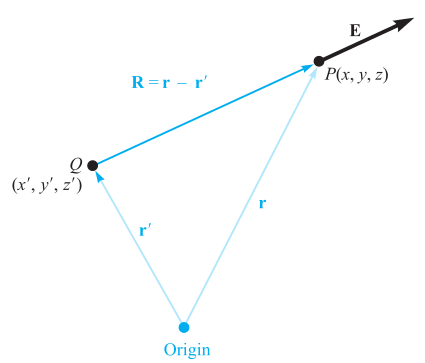
\includegraphics[scale=0.5]{img/referentiel.png}
	\caption{Référentiel quelconque.}
	\label{fig:referentiel}
\end{figure}

\section{Densité de flux électrique, loi de Gauss et divergence}
\subsection{Champ de déplacement électrique}
Le champ de déplacement électrique ou densité de flux
électrique est donné par
\begin{equation}
	\D = \perm \E
	\u{\coulomb\per\meter\squared}
	\label{eq:def-d}
\end{equation}

\subsection{Loi de Gauss}
\begin{mylaw}
Le flux électrique à travers une surface
fermée est égal à la quantité de charge située à
l'intérieur de cette surface fermée.
\end{mylaw}

Mathématiquement,
\begin{equation}
	\oint_\text{S} \vec{D}_\text{S} \cdot \dif \vec{S} 
	= \int_\text{vol} \rho_v \dif v = Q
	\label{eq:gauss}
\end{equation}

où $\vec{S}$ est défini comme sortant de la surface. 

La loi de Gauss permet de calculer des champs électriques
pour des distribubtions de charges symétriques.

On peut aussi écrire cette équation sous la forme
\begin{equation}
	\divn \D = \rho_v
	\label{eq:gauss-dif}
\end{equation}

en se rappellant de la définition de la divergence.

\begin{mydef}
La divergence d'un vecteur de densité de
flux est égal au flux sortant d'une petit surface
fermée par unité de volume lorsque ce volume tend
vers zéro.
\end{mydef}

Une divergence positive indique donc la présence d'une
\textit{source} tandis qu'une divergence négative indique
la présence d'un \textit{puits}.

On peut passer d'une équation à l'autre en utilisant
le théorème de la divergence
\begin{equation}
	\oint_\text{S} \vec{D}_\text{S} \cdot \dif \vec{S}
	= \int_\text{vol} \divn \D \dif v
\end{equation}

\section{\'{E}nergie et potentiel}
\subsection{Potentiel}
Supposons que l'on veuille déplacer une charge $Q$ d'une
distance $\dif \vec{l}$ dans un champ électrique $\E$.
Par \ref{eq:electric-field}, la force sur cette charge
est
\[ \vec{F}_E = Q\E. \]

La composante de cette force dans la direction
$\dif \vec{l}$ est donc
\[ \vec{F}_{EL} = \vec{F}_E \cdot \hat{a}_l = Q\E\cdot \hat{a}_l. \]

Pour vaincre cette force et déplacer la charge, il
faut appliquer une force
\[ \vec{F}_{appl} = -Q\E \cdot \hat{a}_l. \]

Le travail effectué par une source externe pour
déplacer cette charge d'une distance $\dif l$ est
donc
\[ \dif W = -Q\E \cdot \hat{a}_l \dif l = -Q\E \cdot \dif \vec{l} \]

et le travail total pour déplacer une charge d'un
point $A$ à un point $B$ est donné par
\[ W = -Q \int_A^B \E \cdot \dif \vec{l}. \]

\begin{mydef}
On définit ensuite la \textit{différence de potentiel} $V$
comme le travail effectué (par une source externe) pour
déplacer une charge unitaire positive d'un point à un
autre dans un champ électrique
\begin{equation}
	\Delta V = V_B - V_A = -\int_A^B \E \cdot \dif \vec{l}
	\u{\volt}
	\label{eq:potdef}
\end{equation}
\end{mydef}

Lorsqu'on utilise cette équation, on est souvent amené
à définir une référence de potentiel nul. En général, on
utilise pour cela soit un point de référence représentant
la \textit{terre} soit un point situé à une distance
\textit{infinie} du problème.

\begin{mydef}
Une \textit{surface équipotentielle} est une surface
composée de tous les points ayant le même potentiel.
Toutes les lignes de champ électrique sont perpendiculaires
à cette surface aux points d'intersections. Aucun travail
n'est donc nécessaire pour déplacer une charge sur une
surface équipotentielle.
\end{mydef}

\begin{myprop}
Aucun travail n'est effectué pour déplacer une charge
le long d'un chemin fermé
\begin{equation}
	\oint \E \cdot \dif l = 0.
	\label{eq:E-conservatif}
\end{equation}
Cette équation est valide pour les champs \textit{statique}.
On dit dans ce cas que $\E$ est un champ \textit{conservatif}.
On peut réecrire cette équation comme ceci
\begin{equation}
	\rotn \E = 0
	\label{eq:E-conservatif-dif}
\end{equation}
en utilisant les théorèmes intégraux.
\end{myprop}

Par conséquent, le champ $\E$ dérive d'un potentiel
\begin{equation}
	\E = - \gradn V.
	\label{eq:e-grad-v}
\end{equation}
Cette équation nous permet d'obtenir un peu d'intuition
sur le champ électrique :
\begin{enumerate}
	\item La norme du champ électrique est donnée par la
	valeur maximum de la dérive du potentiel par à la
	distance ;
	\item La direction du champ électrique est opposée
	à la direction dans laquelle le potentiel augmente
	le plus rapidement.
\end{enumerate}

\subsubsection{Potentiel d'une charge ponctuelle}
\begin{equation}
	V = \frac{Q}{4\pi\perm_0}
	\label{eq:pot-charge}
\end{equation}

\subsection{Potentiel d'une distribution de charges}
En utilisant à nouveau le référentiel de la figure
\ref{fig:referentiel}
\begin{equation}
	V(r) = \int_{vol} \frac{\rho_v(r')\dV'}{4\pi\perm_0
	|r-r'|}.
	\label{eq:elec-pot}
\end{equation}

\subsection{Dipôle électrique}
\begin{mydef}
Un dipôle électrique est composé de deux charges ponctuelles
de normes égales mais de signe opposé séparé par une distance
faible par rapport à la distance à laquelle on veut calculer
le champ électrique.
\end{mydef}

\begin{mydef}
On définit le moment du dipole
\begin{equation}
	\vec{p} = Q\vec{d}.
\end{equation}
\end{mydef}

Pour trouver le champ électrique et le potentiel électrique
d'un dipôle, on commence par trouver le potentiel dû aux
deux charges via \ref{eq:pot-charge} et on utilise
ensuite l'approximation de Fraunhofer (comme en physique 3
pour les ondes) pour trouver ce même potentiel à une
grande distance du dipôle. On utilise ensuite l'équation
\ref{eq:e-grad-v} pour trouver le champ électrique.
C'est une bonne illustration de comment utiliser le
potentiel pour simplifier les calculs. De plus, cela
justifie la méthode des images (voir sous-section
\ref{subseq:images}).

\subsection{Dénsité d'énergie}
\begin{equation}
	W_E = \frac{1}{2} \int_{vol} \D \cdot \E \dif v
	= \frac{1}{2} \int_{vol} \perm_0\E^2 \dif v
\end{equation}

\section{Conducteurs et diélectriques}
\subsection{Courant et densité de courant}
\begin{mydef}
Un mouvement de charge constitue un \textit{courant}
\begin{equation}
	I \eqdef \fdif{Q}{t}.
	\u{\ampere}
	\label{eq:current}
\end{equation}
Le courant est donc défini comme un mouvement de charge
positive.
\end{mydef}

\begin{mydef}
La densité de courant est définie par
\begin{equation}
	\J \eqdef \frac{\Delta I}{\Delta S} \hat{\mu}_n
	\u{\ampere\per\meter\squared}
	\label{eq:current-density}
\end{equation}
où $\hat{\mu}_n$ est normal à $\Delta S$ dans la
direction du courant. On peut donc réecrire
le courant comme
\begin{equation}
	I = \int_S \J \cdot \dif \vec{S}.
\end{equation}

% A CONFIRMER (même si ça semble relativement logique)
\begin{myrem}
Attention : alors qu'on définissait $\dif \vec{S}$ comme
sortant de la surface pour la Loi de Gauss, ici $\dif \vec{S}$
est défini dans le sens du courant.
\end{myrem}

\begin{myrem}
Imaginons qu'un courant circule dans une feuille d'épaisseur
infinitisémale, dans ce cas, $\J$ est infini. On définit
dans ce cas la densité de courant surfacique $\K [\si{\ampere
\per\meter}]$ comme illustré sur la figure \ref{fig:current-surface-density}. Si $\K$ est uniforme, on a
\begin{equation}
	I = Kb
\end{equation}
où $b$ est mesuré perpendiculaire à la direction du courant.
Si $\K$ n'est pas uniforme, on a cette fois
\begin{equation}
	I = \int K \dif N
\end{equation}
où $\dif N$ est perpendiculaire à la direction du courant.
\end{myrem}

\begin{figure}[ht]
	\centering
	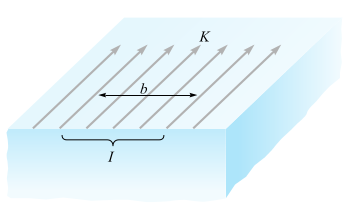
\includegraphics[scale=0.5]{img/current-surface-density.png}
	\caption{Illustration de la densité de courant
	surfacique $\K$.}
	\label{fig:current-surface-density}
\end{figure}

\end{mydef}
A partir de l'équation \ref{eq:current}, on peut écrire
\[ \Delta I = \frac{\Delta Q}{\Delta t} = \rho_v\Delta S
\frac{\Delta x}{\Delta t} = \rho_v\Delta S v_x \]
et donc via \ref{eq:current-density}
\begin{equation}
	\J = \rho_v\vec{v}
	\label{eq:convection}
\end{equation}
ce qui montre bien qu'un mouvement de charge constitue
un courant. Ce type de courant s'appelle un \textit{courant
de convection}.

\subsection{Continuité du courant}
% Not really a 'law', more a 'principle'
\begin{mylaw}[Conservation de la charge]
Une charge électrique ne peut ni être créée ni détuite.
\end{mylaw}

De ce principe de conservation de la charge,
on peut écrire
\begin{equation}
	I = \oint_S \J \cdot \dif S = - \fdif{Q_i}{dt}
\end{equation}
où $Q_i$ représente la charge située dans la
surface fermée.

En utilisant le théorème de la divergence, on
peut à nouveau réécrire cette équation sous forme
différentielle
\begin{equation}
	\divn \J = - \fpart{\rho_v}{t}
	\label{eq:cont-cur-dif}
\end{equation}

\subsection{Conducteur métallique}
Dans un conducteur métallique, les électrons ont
une vitesse moyenne qu'on appelle la vitesse de
dérive $\vec{v}_d$. Les cours de dispositifs nous
montre que
\begin{equation}
	\vec{v}_d = -\mu_e\E
	\label{eq:driftv}
\end{equation}
où $\mu_e$ est le mobilité des électrons mesurées
en \si{\meter\squared\per\volt\per\second}. En injectant
\ref{eq:driftv} dans \ref{eq:convection} on obtient
\begin{equation}
	\J = -\rho_e\mu_e\E
\end{equation}
où $\rho_e$ est la densité des charges des électrons (et
donc est négatif). On définit la \textbf{conductivité}
\begin{equation}
	\sigma = -\rho_e\mu_e
	\u{\siemens\per\meter}
\end{equation}
telle que
\begin{equation}
	\J = \sigma \E
\end{equation}
et la résistivité $\rho = \sigma^{-1}$.

\begin{myrem}
Cette dernière équation couplé à l'équation de
continuité du courant \ref{eq:cont-cur-dif} dans
un cas statique
\begin{equation}
	\divn (\sigma \E) = 0
\end{equation}
permet parfois d'obtenir des informations sur
$\E$ lorsque l'injection de l'ansatz dans les
équations de Maxwell ne donne rien\footnote{C'est
le cas par exemple si \ref{eq:E-conservatif-dif}
donne $0 = 0$ et si $\rho_v$ dans \ref{eq:gauss-dif}
est non-constant (voir footnote \ref{foot:rho}) et inconnu.}.
\end{myrem}

On définit également la résistance
\begin{equation}
	R \eqdef \frac{V_{ab}}{I} = 
	\frac{-\int_b^a \E \cdot \dif \vec{l}}{\int_S \sigma\E \cdot
	\dif \vec{S}}
	\u{\ohm}
\end{equation}
où $V$ est la différence de potentiel entre deux surfaces
équipotentielles du matériau et $I$ le courant total
traversant la surface la plus positive du matériau.

\subsection{Méthodes des images}
\label{subseq:images}
Le potentiel électrique causé par un dipôle électrique
présente la particularité d'être nul sur le plan à mi-
chemin entre les deux charges électriques qui constituent
le dipôle. Un tel plan équipotentiel à $V = 0$ peut être
représenté par une plaque conductrice infinie.
Comme illustré sur la figure \ref{fig:image1},
on peut donc passé d'une charge au-dessus d'une plaque
conductrice à deux charges opposées sans plaque
conductrice (et vice-versa) sans que les champs
de la partie supérieur du système changent.
La charge ajoutée ajoutée est appelée charge \textit{image}.

\begin{figure}[ht]
	\centering
	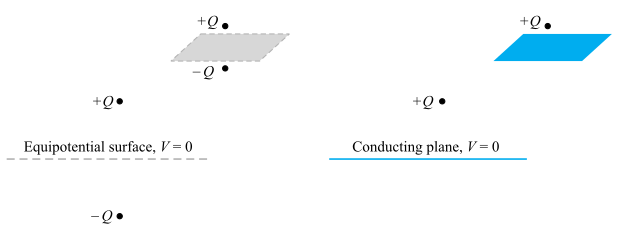
\includegraphics[scale=0.6]{img/image1.png}
	\caption{Méthode des images simple.}
	\label{fig:image1}
\end{figure}

Par linéarité, on peut répéter ce procédé encore et
encore comme illustré sur la figure \ref{fig:image2}. 

\begin{figure}[ht]
	\centering
	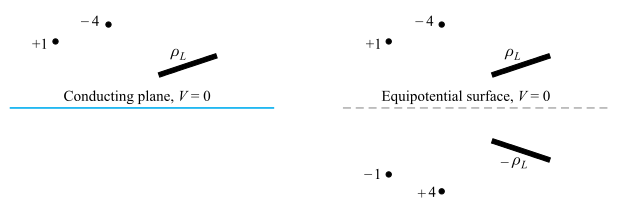
\includegraphics[scale=0.6]{img/image2.png}
	\caption{Méthode des images par linéarité.}
	\label{fig:image2}
\end{figure}

Dans plusieurs cas, le potentiel électrique du nouveau
système obtenu est plus simple à calculer puisqu'il ne
contient plus de plaque conductrice infinie avec une
densité de surface inconnue.

\subsection{Conducteur électrique parfait et conditions aux interfaces}
\begin{myprop}
Un conducteur électrique parfait possède les propriétés
suivantes :
\begin{enumerate}
	\item La densité de charge à l'intérieur du conducteur
	est nulle ;
	\item Toutes les charges se trouvent sur la surface du
	conducteur.
\end{enumerate}
En électrostatique (pas de courant), on a en plus
\begin{enumerate}
	\item Le champ électrique à l'intérieur du conducteur
	est nul ;
	\item Le champ tangentiel à la surface est nul.
\end{enumerate}
\end{myprop}

Mathématiquement, en appliquant \ref{eq:E-conservatif} sur
le chemin rectangulaire de la figure \ref{fig:conductor-boundary},
on trouve bien que la composante tangentielle de $\E$ est nulle
\begin{equation}
	\E \times \hat{n} \Big|_s = 0.
	\label{eq:cci-1}
\end{equation}
En appliquant \ref{eq:gauss} sur le cylindre de
la figure \ref{fig:conductor-boundary}, on trouve une
relation entre la composante normale à la surface et
la densité de charge du conducteur
\begin{equation}
	\D \cdot \hat{n} \Big|_s = \rho_s
	\label{eq:cci-2}
\end{equation}
Dans ces deux équations, $\hat{n}$ est le vecteur unitaire
normal au conducteur et \textbf{sortant} du conducteur.

\begin{figure}[ht]
	\centering
	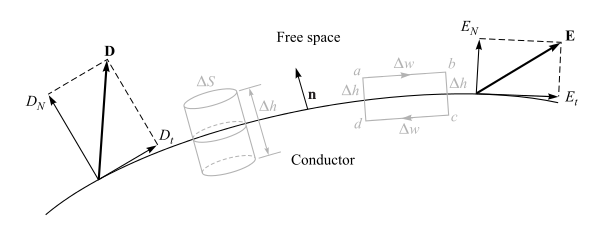
\includegraphics[scale=0.6]{img/conductor-boundary.png}
	\caption{Conditions limites pour un conducteur parfait.}
	\label{fig:conductor-boundary}
\end{figure}

% TODO : MATÉRIAUX DIÉLECTRIQUES
\subsection{Diélectrique parfait et conditions aux interfaces}
En appliquant \ref{eq:E-conservatif} sur le chemin rectangulaire
de la figure \ref{fig:dielectric-boundary}, on trouve que le
le champ $\E$ tangentiel est continu aux interfaces
\begin{equation}
	(\E_1 - \E_2) \times \hat{n} = 0
\end{equation}
et donc automatiquement que le champ $\D$ tangentiel est
discontinu aux interfaces.

En appliquant \ref{eq:gauss} sur le cylindre de
la figure \ref{fig:dielectric-boundary}, on trouve
\begin{equation}
	(\D_1 - \D_2) \cdot \hat{n} = \rho_s
\end{equation}
où $\rho_s$ est la quantité de charge libre sur l'interface
(très souvent\footnote{\label{foot:rho}En fait il n'y a que deux cas pour
lequel la densité de charge dans un diélectrique (que ce soit
en surface ou en volume) n'est pas nulle. Le premier cas est celui
ou des charges ont été implantées dans le diélectrique isolant
(dopage). Le deuxième cas est celui la conductivité est
variable.} 0).
Dans ces deux équations, $\hat{n}$ est le vecteur normal
à l'interface allant de la région 2 vers la région 1.

\begin{myrem}
On remarque que les conditions aux interfaces \ref{eq:cci-1}
et \ref{eq:cci-2} sont en fait des cas particuliers de
ces conditions pour $\E_2 = \D_2 = \vec{0}$.
\end{myrem}

\begin{figure}[ht]
	\centering
	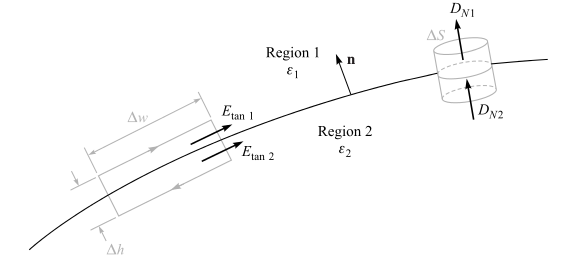
\includegraphics[scale=0.6]{img/dielectric-boundary.png}
	\caption{Conditions limites pour un diélectrique parfait.}
	\label{fig:dielectric-boundary}
\end{figure}

\section{Capacitance}
\begin{mydef}
La \textit{capacitance} de deux conducteurs portant
des charges opposés $Q$ et $-Q$ et dont
la différence potentiel est $V_0$ est définie comme
\begin{equation}
	C \eqdef \frac{Q}{V_0}
	\u{\farad}
\end{equation}
\end{mydef}

En utilisant \ref{eq:gauss} et \ref{eq:potdef}, on
obtient
\begin{equation}
	C = \frac{\oint_S \perm\E \cdot \dif \vec{S}}{
	-\int_-^+ \E \cdot \dif \vec{L}}
\end{equation}

\begin{myrem}
Lorsqu'on utilise cette dernière équation pour calculer
une capacitance, il faut faire attention. Lorsqu'on charge
une capacité, la somme totale des charges réparties dans
la capacité est nulle. Pour utiliser la dernière équation,
il ne faut donc considérer que les charges positives ou les
charges négatives (et si possible choisir le cas le plus
simple pour appliquer Gauss).
\end{myrem}

Pour une capacitance constitué de deux plaques
parallèles de surface $S$ et séparé par une distance
$d$, on a
\begin{equation}
	C = \frac{\perm S}{d}.
\end{equation}
L'énergie stockée dans cette capacitance est
donné par
\begin{equation}
	W_E = \frac{1}{2}CV^2 = \frac{1}{2}QV =
	\frac{1}{2}\frac{Q^2}{2C}.
	\label{eq:energie-capa}
\end{equation}
\subsection{\'{E}quations de Laplace et de Poisson}
L'équation de Poissonpermet d'obtenir un potentiel
en connaissant les valeurs de ce potentiels aux frontières
du problème. Elle s'obtient très facilement en utilisant
\ref{eq:gauss-dif}, \ref{eq:def-d} et \ref{eq:e-grad-v}
\[ \divn \D = \divn (\perm \E) = -\divn (\perm \gradn V) = \rho_s \]
ce qui peut finalement se réecrire
\begin{equation}
	\lap V = -\frac{\rho_v}{\perm}.
\end{equation}
Cette équation est valide pour une région homogène
dans laquelle $\perm$ est constant. Si $\rho_v = 0$,
l'équation de Poisson devient l'équation de Laplace
\begin{equation}
	\lap V = 0.
\end{equation}

\begin{mytheo}[Existence et unicité]
La solution d'une équation de Poisson dont les
conditions aux limites sont appropriées existe et
est unique.
\end{mytheo}

Ce théorème permet de justifier le fait que changer
le problème sans changer ses conditions aux limites
(grâce à la méthode des images par exemple) nous
fournit bien l'unique solution.

On peut résoudre une équation de Laplace par
séparation de variables (voir cours de mathématique 3).

% TODO: à faire relire
\subsection{Travaux virtuels}
Le principe des travaux virtuels s'applique aux systèmes
isolés énergétiquement de l'extérieur, autrement dit 
aux systèmes dont l'énergie est conservée.

Pour mieux comprendre, prenons un exemple insipiré
d'un correctif d'APE.

Imaginons que l'on veuille connaître la force s'exerçant sur
une plaque d'un condensateur isolé pour lequel $Q$ est constant.
On va virtuellement tirer (ou pousser) sur cette plaque et
voir comment le système réagit afin de mesurer cette force.
On considère donc un déplacement infinitésimal d'une plaque d'un
condensateur. Si une force s'exerce sur cette plaque, cela
signifie qu'une certaine énergie peut-être récupérée lors
de ce déplacement (si on rapproche les plaques) ou doit être
fournie pour pemettre ce déplacement (si on éloigne les plaques).
\[ \dif W_m = \vec{F} \cdot \vec{\dif l}. \]
Cette énergie retirée ou ajoutée au système doit être stockée
sous forme d'énergie électrique ou magnétique. Le changement
de géométrie du condensateur entraîne une différence
d'énergie. Si la charge $Q$ est constante, cette différence
est donnée par (en utilisant \ref{eq:energie-capa})
\[ \dif W_e = \fpart{}{C}\left(\frac{Q^2}{2C}\right) =
\frac{Q^2}{2} \fpart{}{x}\left(\frac{1}{C(x)}\right). \]
On peut finalement écrire le bilan d'énergie
\[ \dif W_e = \dif W_m. \]
Si maintenant on relâche cette plaque, elle retournera à sa
position initiale en libérant (ou absorbant) toute
l'énergie $W_e$ stockée précédemment en subissant une
force $F_x$ dont la direction est opposé à celle qu'on
avait nous même virtuellement appliqué
\[ F_x = - \frac{Q^2}{2} \fpart{}{x}\left(\frac{1}{C(x)}\right). \]

De manière générale, on a pour un condensateur isolé
avec une charge $Q$ constante
\begin{center}
\textit{énergie mécanique fournie $=$ variation d'énergie du système}
\end{center}
et pour un condensateur raccordé à une source de
tension (pour maintenir $V$ constant)
\begin{center}
\textit{énergie fournie par la batterie $+$ énergie mécanique fournie
$=$ variation d'énergie du système}.
\end{center}

\part{Magnétostatique}
\section{Champ magnétique constant}
\subsection{Loi de Biot-Savart}
La loi de Biot-Savart en magnétostatique et l'analogue
de la loi de Coulomb en électrostatique.
\begin{mylaw}
Expérimentalement, on peut montrer qu'un champ magnétique
est produit par un courant continu $I$ circulant dans un élément
de longueur infinitésimal $\dl$ et vaut
\begin{equation}
	\vec{\dif H} = \frac{I\dl \times a_r}{4\pi R^2}.
	\u{\ampere\per\meter}
\end{equation}
Son sens est donné par la règle du tire-bouchon de la
main droite.
\end{mylaw}

On peut réecrire cette équation en utilisant la définition
de densité de courant
\begin{equation}
	\H = \int_{vol} \frac{\J \times \hat{a}_r}{4\pi R^2}\dV
\end{equation}

\subsection{Loi d'ampère}
\begin{mylaw}
L'intégrale du champ $\H$ sur un chemin fermé est égale
au courant ``passant'' dans ce chemin fermé
\begin{equation}
	\oint \H \cdot \dl = \int_{in} \J \cdot \dS = I.
\end{equation}
\end{mylaw}
En utilisant le théorème de Stoke, on peut écrire cette
dernière équation sous forme différentielle\footnote{Une
interprétation très intuitive du rotationnel se trouve
à la page 199 du livre.}
\begin{equation}
	\rotn \H = \J.
\end{equation}

\subsection{Flux magnétique et densité de flux magnétique}
\begin{mydef}
On définit la \textit{densité de flux magnétique} dans
le vide
\begin{equation}
	\B = \mu_0\H.
	\u{\tesla = \weber\per\meter\squared}
\end{equation}
\end{mydef}

\begin{mydef}
On définit maintenant le flux magnétique
\begin{equation}
	\Phi = \int_S \B \cdot \dS.
	\u{\weber}
\end{equation}
\end{mydef}

\begin{mylaw}[Loi de Gauss pour le champ magnétique]
La loi de Gauss pour le champ électrique stipulait
que le flux sortant d'une surface fermée devait provenir
d'une source (c'est à dire une charge) situé à l'intérieur
de cette surface fermée. Pour un champ magnétique, les lignes
de champs bouclent toujours sur elles-même, il n'y a pas
de monopôle magnétique
\begin{equation}
	\oint \B \cdot \dS = 0.
\end{equation}
En utilisant le théorème de la divergence, on obtient
\begin{equation}
	\divn \B = 0.
	\label{eq:gauss-magn-dif}
\end{equation}
\end{mylaw}

\subsection{Potentiel scalaire et potentiel vecteur magnétique}
% Besoin de faire le potentiel scalaire?
\subsubsection{Potentiel vecteur}
En utilisant l'équation \ref{eq:gauss-magn-dif} et en
se rappellant que la divergence d'un rotationnel est toujours
nulle, on peut écrire
\begin{equation}
	\B = \rotn \A
\end{equation}
où est $\A~\si{[\weber\per\meter]}$ est-ce qu'on appelle
un \textit{potentiel vecteur magnétique}. Jusqu'ici on a
juste définit $\A$ comme un vecteur qui respecte les équations
obtenues précédemment. On peut déterminer $\A$ en
utilisant la loi de Biot-Savart, la définition de $\A$
et la définition de $\B$, on peut montrer que
\begin{equation}
	\A = \oint \frac{\mu_0 I\dl}{4\pi R}
\end{equation}
ce qui en comparaison avec l'équation \ref{eq:elec-pot}
ressemble bien à un potentiel. A nouveau, on peut utiliser
la définition de densité de courant pour réecrire cette
équation sous la forme
\begin{equation}
	\A = \int_vol \frac{\mu \J}{4\pi R}\dV.
\end{equation}

\part{Lignes de transmission}

\part{Guides d'ondes}

\end{document}
